\chapter*{Annexes}

\annexe{Terminologie}{terminologie}
\printglossaries

\annexe{Sujet du stage}{annexeSujetStage}
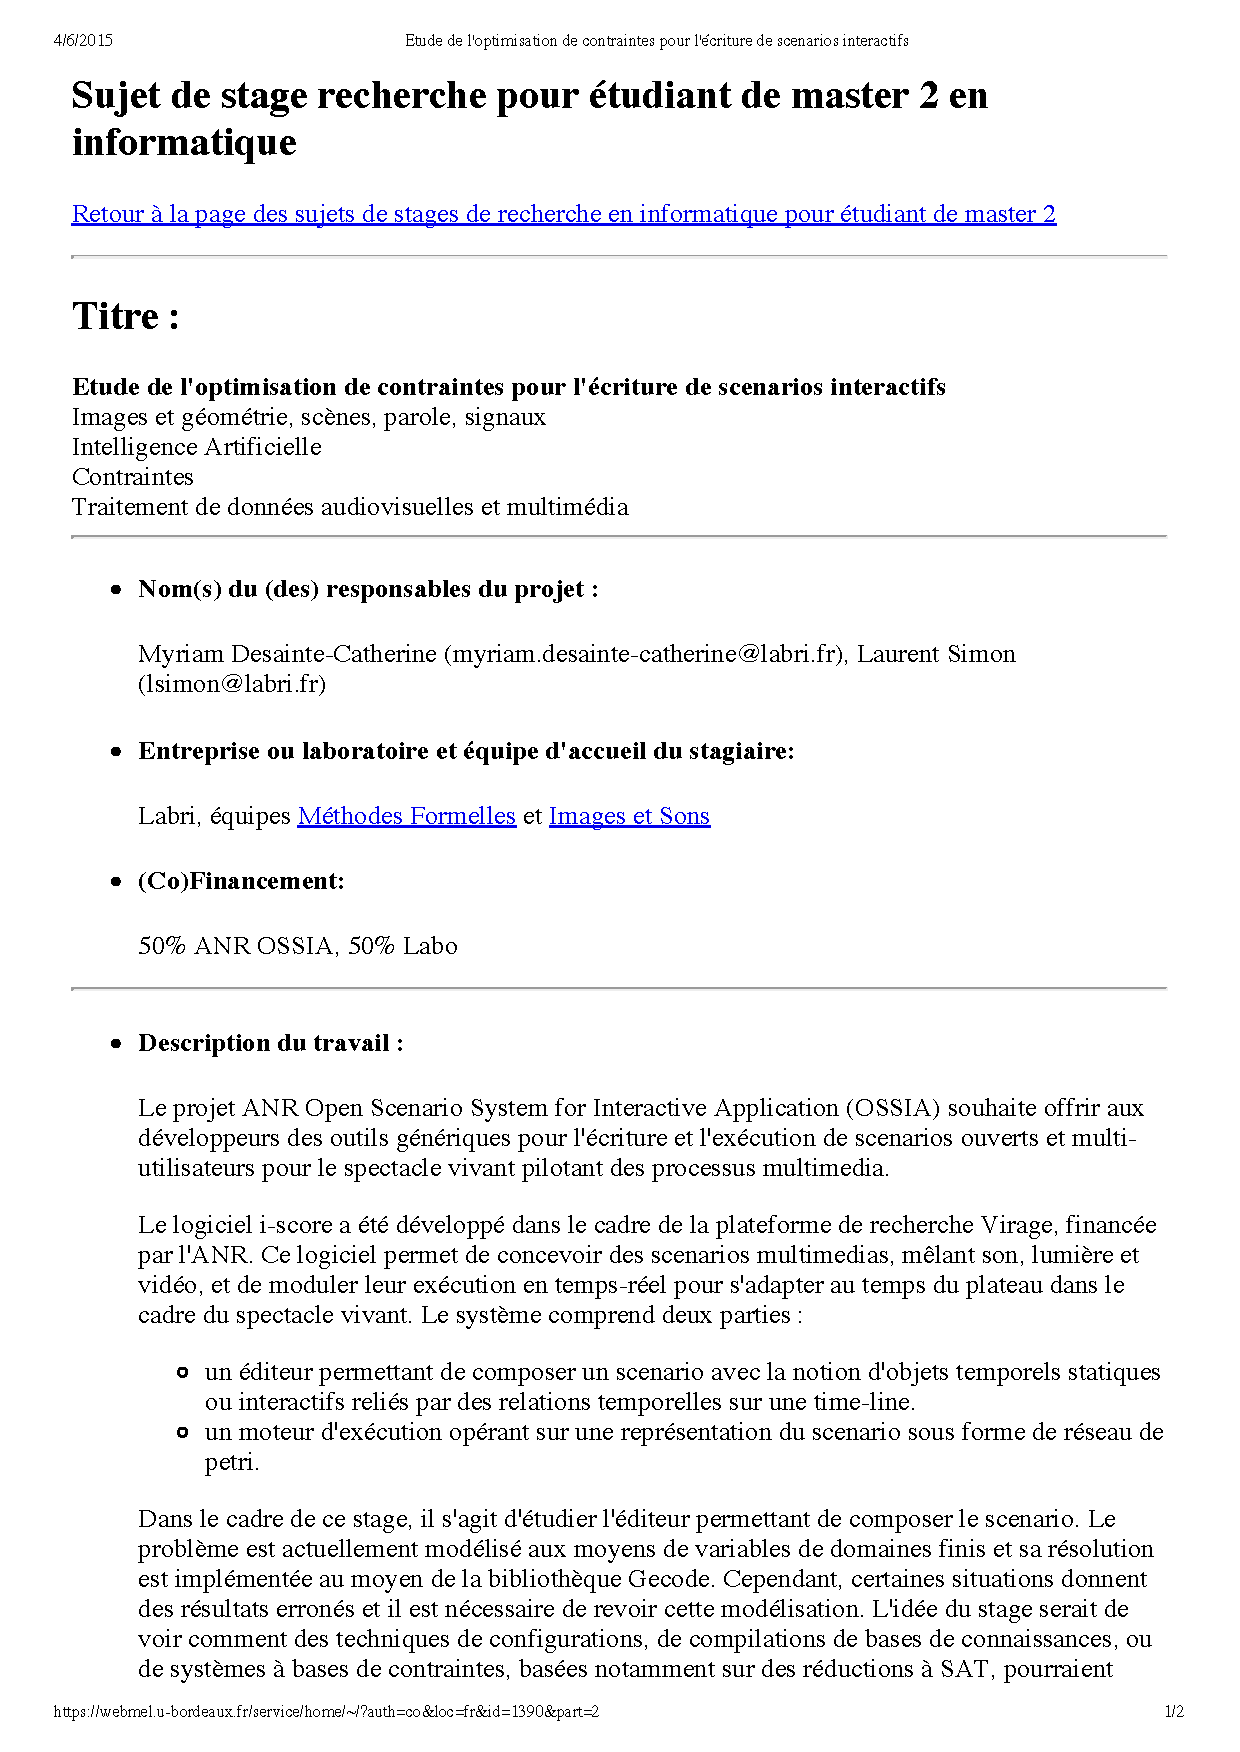
\includepdf[pages={1-2}]{ressources/sujetStage}

\annexe{Éxemple du puzzle Cryptarithmétique avec \ortools}{annexePuzzle}
\inputminted{cpp}{ressources/cryptarithm.cpp}

\annexe{L'historique d'\iscore}{annexeHistorique}
\schema{HeritageI-scoreNew}{L'évolution d'\iscore{} et les solveurs utilisés. Image tirée de \url{http://web.archive.org/web/20150404094549/http://i-score.org/development/}.}

\annexe{Document de proposition 1}{annexeIncoherences}
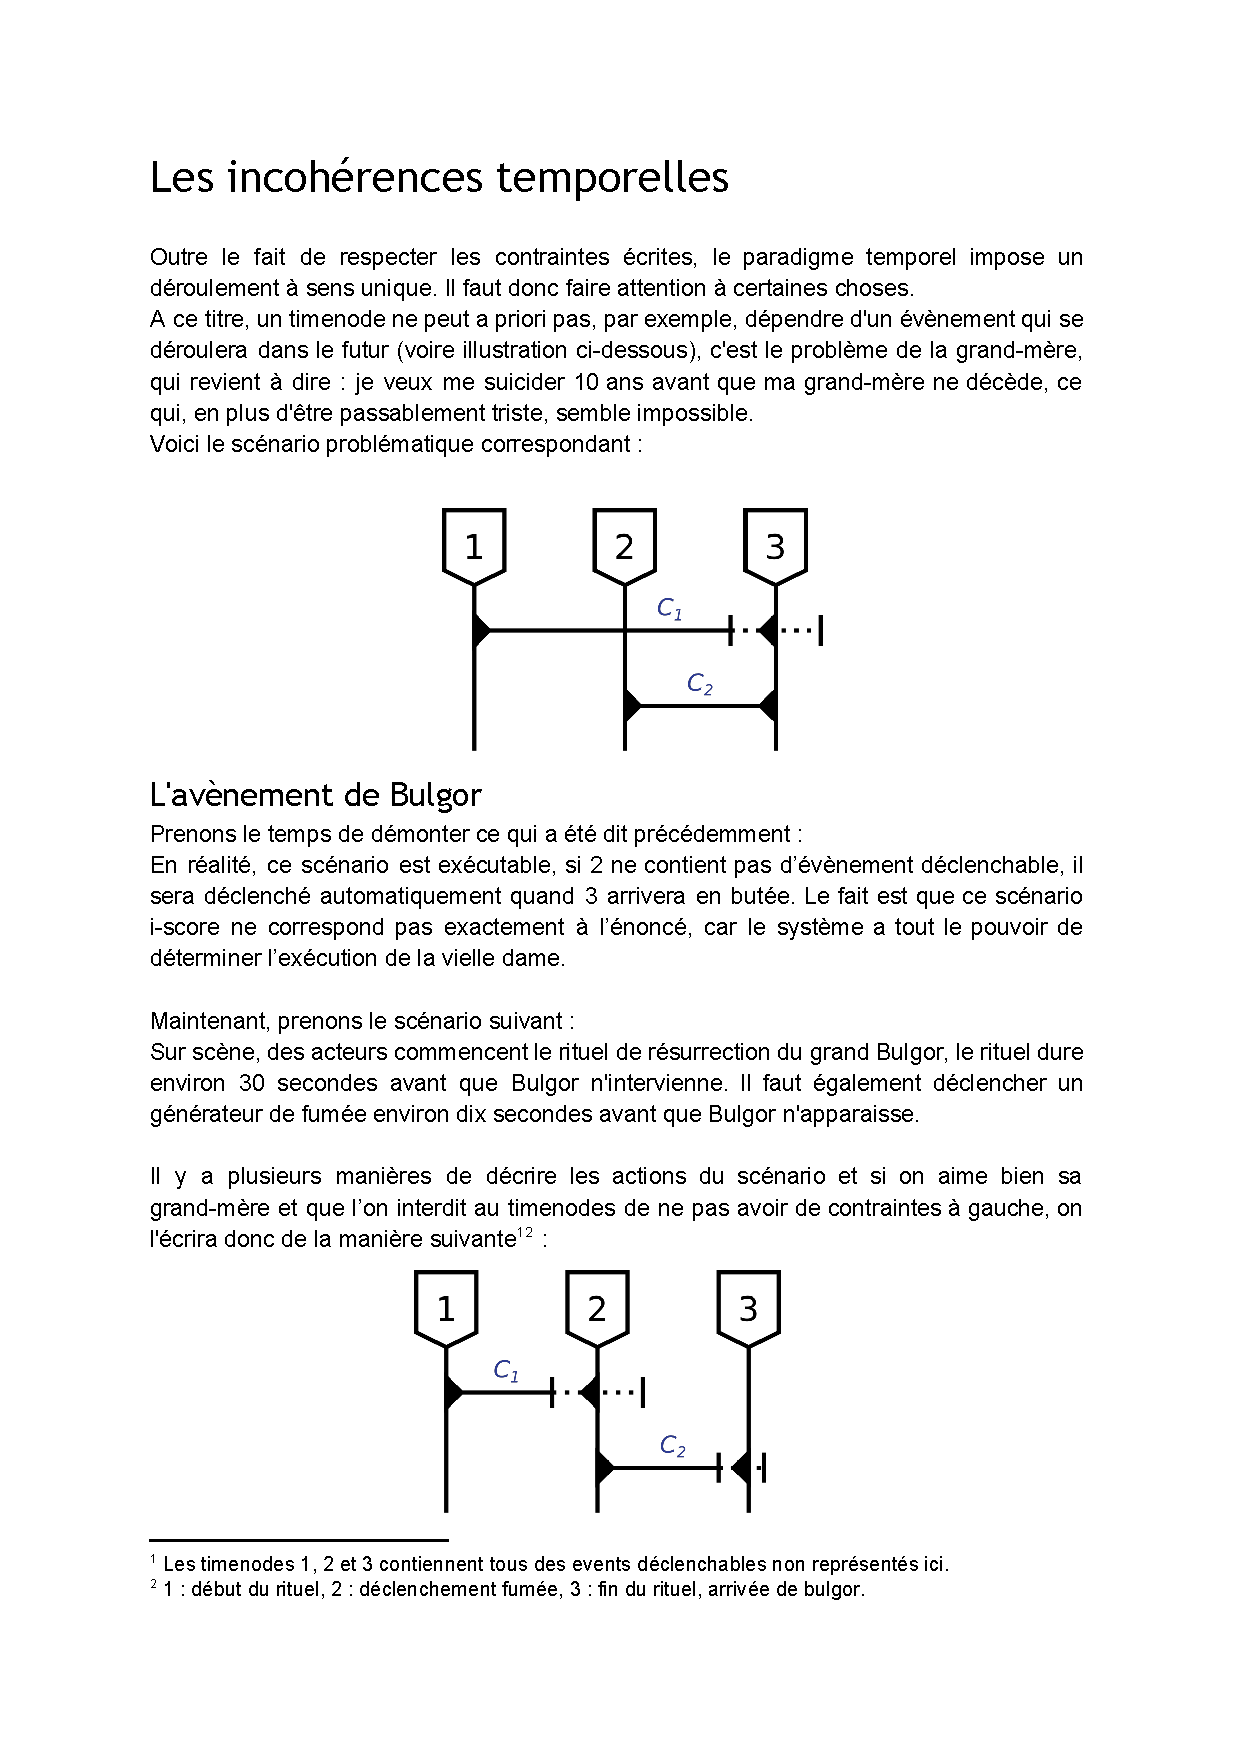
\includepdf[pages={1-2}]{ressources/lesIncoherencesTemporelles}

\annexe{Document de proposition 2}{annexeStartnode}
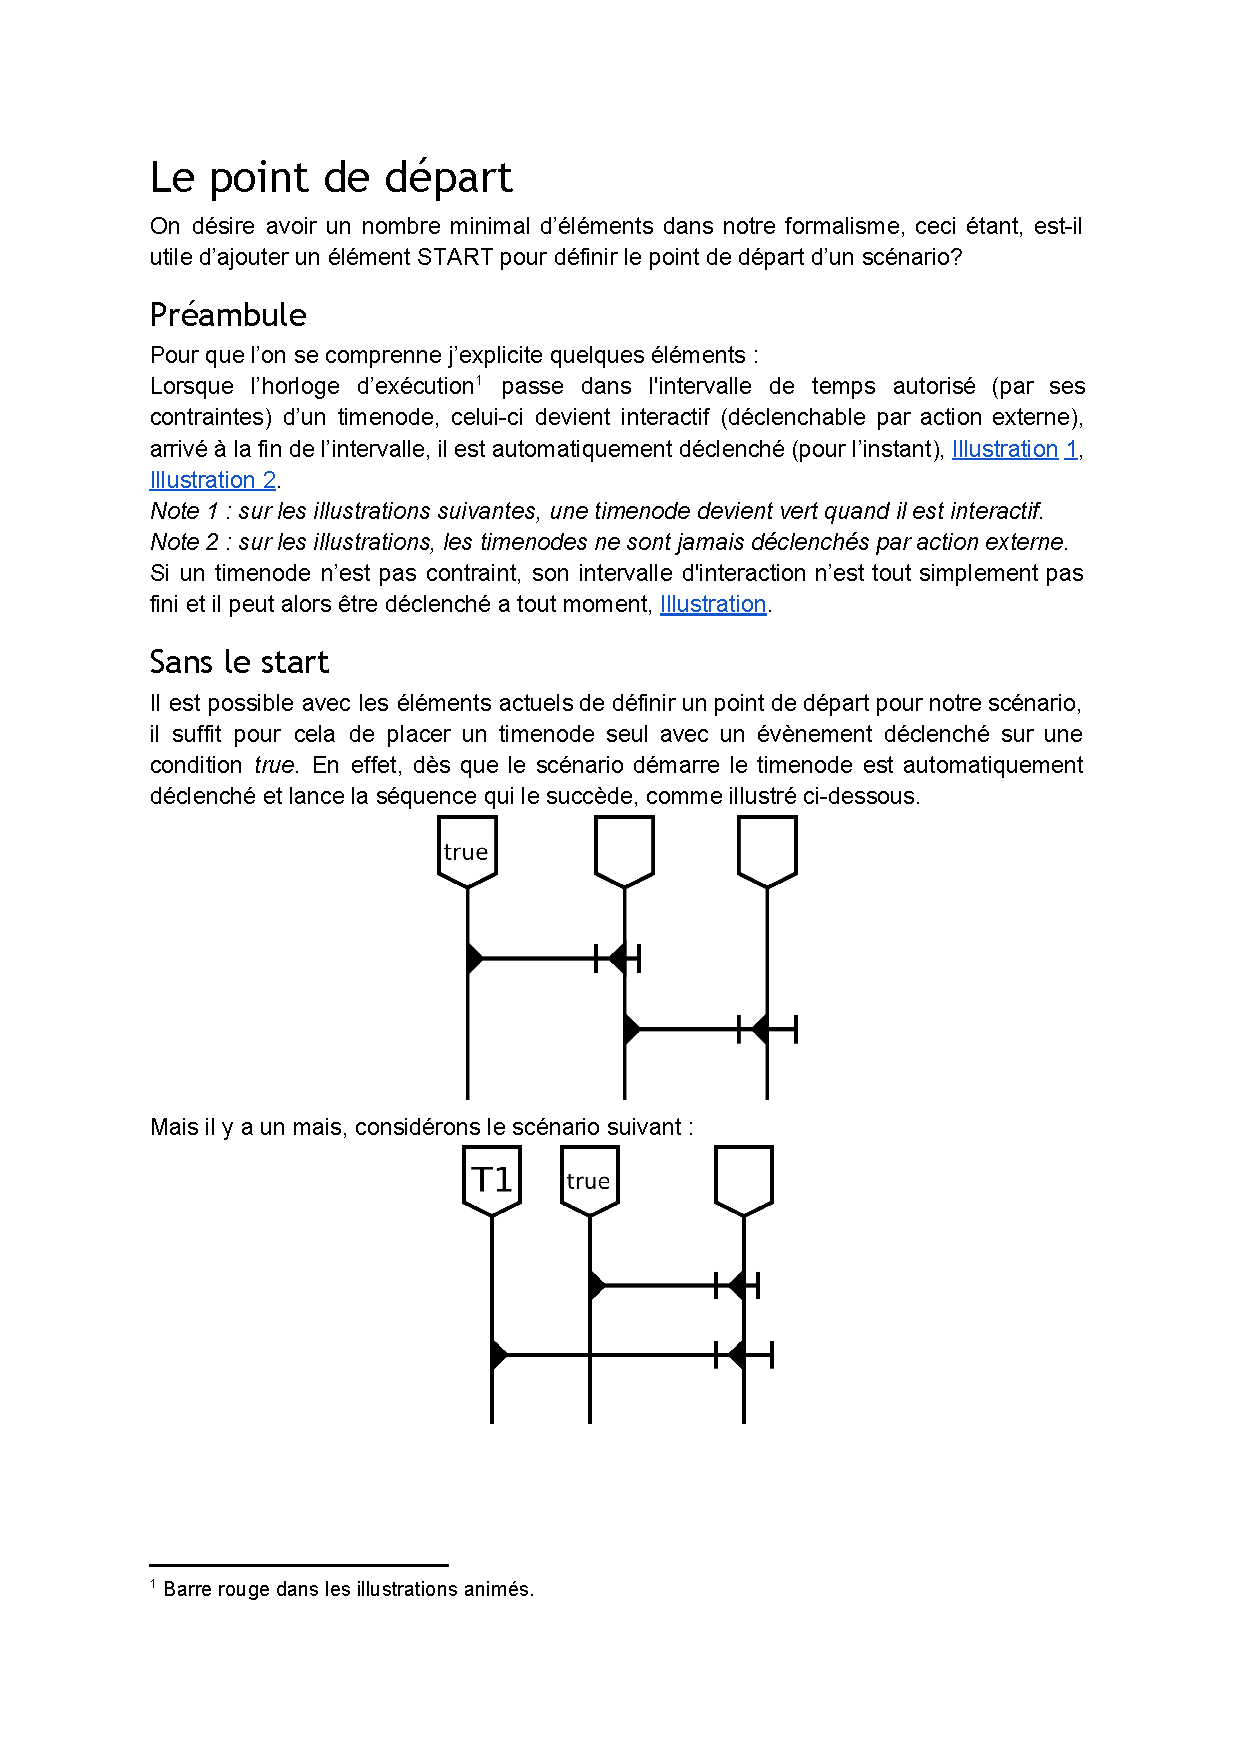
\includepdf[pages={1-3}]{ressources/leStartnode}